\section{FlakeAgent}
\label{sec:approach}

\subsection{Overview}

Figure~\ref{fig:overview} shows the architecture of FlakeAgent. The agent
consists of four components: (i) an \emph{observation probe} that runs Maven
invocations locally and compresses their outcome into a structured
observation; (ii) a \emph{strategy space} of twelve executor-side execution
schemes, each parameterized by a small, type-checked JSON schema; (iii) a
\emph{planner} (an LLM) that, each round, forms a causal hypothesis about the
flakiness mechanism and selects one strategy with parameters; and (iv) a
\emph{diagnoser} (the same LLM, invoked once after a failure is reproduced)
that emits a category label, a root-cause hypothesis, and file--line evidence.
All LLM calls go through vendor APIs; no model is deployed locally.

\begin{figure}[t]
\centering
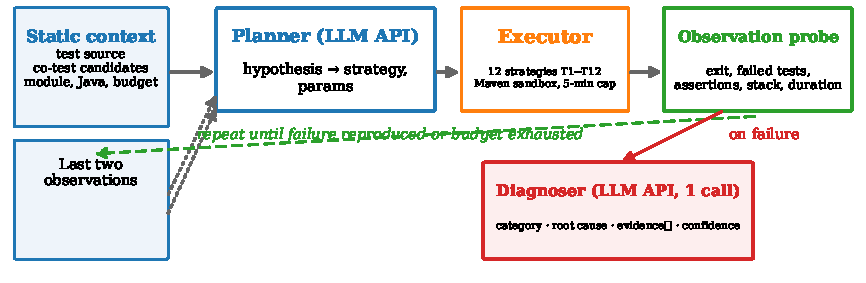
\includegraphics[width=0.95\columnwidth]{figures/overview.pdf}
\caption{Overview of FlakeAgent. Step~0 runs three baseline isolated reruns
(no LLM). Each planning round feeds the LLM a bounded context — the test
source, the module's candidate co-tests, and the last two structured
observations — and it returns a JSON plan \texttt{\{strategy, params,
hypothesis, expected\}}. The executor implements the chosen strategy locally,
the probe compresses the run into a structured observation, and the loop
repeats until a failure is reproduced or the budget (6 LLM calls, 8
executions, 45 minutes) is exhausted. On a reproduced failure, one diagnose
call emits \texttt{\{category, root\_cause, evidence[], confidence\}}, which
we evaluate against the developer fix commit.}
\label{fig:overview}
\end{figure}

The loop is deliberately \emph{closed}: the planner only ever sees (a) static
context (test source, candidate co-tests, build metadata) and (b) the
structured results of executions it requested. It never sees the ground-truth
category, the developer fix, or any failure log produced elsewhere — the
cold-start condition we evaluate in Section~\ref{sec:results}. All twelve
strategies are implemented executor-side; the LLM only selects a strategy
identifier and its parameters, which a sanitizer coerces into safe ranges
(Section~\ref{sec:antideg}). This division of labor has three benefits: the
executions are deterministic and auditable; the LLM cannot hallucinate
commands or touch the filesystem; and the strategy semantics are documented
once, in code, so the prompt only needs to explain \emph{when} each strategy
applies, not \emph{how} to run it.

\subsection{The observation probe}

Every execution — whether from the agent loop, the baselines
(Section~\ref{sec:setup}), or the validation gate — passes through one probe,
\texttt{run\_mvn}, which executes Maven/Surefire in a local sandbox
(project snapshot at the flaky commit, offline Maven repository at the
snapshot's dependency cache, Java version pinned per project) and parses the
result into a structured observation:

\begin{lstlisting}[style=jsonsmall,label=lst:obs]
{"strategy": "T6", "params": {"sleep_ms": 500, "target_method": "waitUntil"},
 "exit_code": 0, "duration_s": 41.2,
 "failed": [{"name": "pkg.Class#testA", "message": "expected: 100 but was: 200",
             "stack": "pkg.Class.java:460 -> ..."}],
 "passed": 3, "error": null, "log_tail": "...", "subruns": null}
\end{lstlisting}

The probe extracts, from Surefire XML reports and console output: the set of
failed test names with assertion messages and stack traces, the number of
passing tests, the wall-clock duration, and a bounded tail of the raw log.
For the same-JVM double-run strategy (T2), whose plugin (iDFlakies'
\texttt{testrunner}) reports per-sub-run results in its own JSON files, the
probe additionally attaches a \texttt{subruns} list with the outcome of each
execution of the test inside the shared JVM — the signal that distinguishes
``passes every time alone, fails on the second run in one JVM'' from a plain
rerun failure. A failure of the target test is defined as an entry in
\texttt{failed} whose name matches the target class or method; for T2 we
match against the per-sub-run entries. The probe treats the observation as
failing only when the \emph{target} test fails — failures of unrelated
co-tests during order-based strategies are recorded in the log but do not
count as reproduction.

\subsection{The strategy space}

Table~\ref{tab:strategies} lists the twelve strategies. They span the four
flakiness categories and the execution conditions each category's mechanism
requires. Strategies are grouped into four families that the anti-degeneracy
rules (Section~\ref{sec:antideg}) reason about: \emph{order} (T3, T4, T5,
T10), \emph{timing/resource} (T6, T7, T8, T9), \emph{nondeterminism} (T12),
and \emph{amplification} (T1, T2). Notably, the space includes two
\emph{deliberate} execution schemes that no rerun loop would ever try: T2
(run the test twice back-to-back in one JVM via the iDFlakies
\texttt{testrunner} plugin, the dataset's own NIO mechanism) and T12 (perturb
JVM nondeterminism with NonDex). Both are essential: T2 is the only strategy
that can expose non-idempotent self-pollution, and T12 is the only one that
can trigger implementation-dependent failures at will.

\begin{table}[t]
\caption{The twelve executor-side strategies. Parameters are chosen by the
LLM and coerced by the sanitizer into the listed ranges. ``Target'' is the
flakiness category the strategy is designed to expose (the agent is never
told this).}
\label{tab:strategies}
\small
\begin{tabular}{@{}llp{4.1cm}ll@{}}
\toprule
\textbf{ID} & \textbf{Strategy} & \textbf{Mechanism} & \textbf{Params (range)} & \textbf{Target}\\
\midrule
T1 & rerun-isolated & plain reruns in fresh JVMs & repeats (1--3) & TD (rare)\\
T2 & same-JVM double-run & test run $k$ times consecutively in one JVM via testrunner plugin & runs (2--4) & NIO\\
T3 & order-permutation & chosen co-tests run before the test, fixed order & cotests ($\le$4 classes) & OD\\
T4 & random-suite-order & full module suite in random order (seeded) & seed & OD\\
T5 & polluter-victim & one chosen polluter, then the test & polluter (1 class or method) & OD\\
T6 & sleep-injection & \texttt{Thread.sleep} injected at method entry, recompiled, reverted after run & sleep\_ms (10--20000), target\_method & TD\\
T7 & system-stress & CPU/IO load during the run & mode, cpus (1--6) & TD\\
T8 & env-manipulation & extra env vars (TZ, LANG, locale) & env (whitelisted keys) & TD/ID\\
T9 & resource-limit & small heap / no fork & xmx, fork\_count & TD\\
T10 & parallel-execution & test class run with parallel methods/classes & threads (2--8) & OD/TD\\
T11 & external-block & hosts blocked via \texttt{/etc/hosts} & hosts ($\le$5) & TD/ID\\
T12 & nondex-seed & NonDex JVM-nondeterminism perturbation & seed, rounds (10--100) & ID\\
\bottomrule
\end{tabular}
\end{table}

Each strategy maps to one Maven invocation with documented Surefire/plugin
flags, e.g.~T3/T5 use \texttt{-Dsurefire.runOrder=testorder} with an explicit
\texttt{-Dtest="A,B"} spec; T4 uses \texttt{runOrder=random} with a seed; T2
uses the iDFlakies \texttt{testrunner:testplugin} goal with the dataset's
exact detector configuration and an \texttt{original-order} file naming the
target test. T6 is the only strategy that touches source code: the executor
injects a \texttt{Thread.sleep} at the entry of a named method
(selected by the LLM), recompiles the module, runs the test, and reverts the
patch in a \texttt{finally} block; the LLM never edits code itself. Sleep
injections are clamped to 20\,s and are, like every strategy, subject to the
same-run dedup rule, which prevents infinite sleep escalation.

\subsection{The plan--execute--observe loop}

The loop proceeds as follows. \textbf{Step 0} (no LLM): the probe runs three
isolated reruns of the target test. Flaky tests sometimes fail on a plain
rerun; when they do, the agent stops immediately with a reproduced failure
and one LLM call saved. \textbf{Planning}: each round, the planner receives a
bounded context — a system prompt describing the task and the JSON contract;
the test identifier, module and Java version; the test class source (up to
two files, 220 lines each, truncated); up to 40 candidate co-test class names
discovered by scanning the module's test tree (usable by T3/T5); the budget
left; and the \emph{last two} structured observations with their assertion
messages. The planner must return one JSON object:
\texttt{\{hypothesis, strategy, params, expected\}}. The hypothesis is a
one-sentence causal claim; \texttt{expected} states what observation would
confirm it. The harness validates the strategy id against the active set,
sanitizes the parameters (Section~\ref{sec:antideg}), executes the strategy
with a 6-minute timeout, and probes the result. \textbf{Termination}: the
loop stops as soon as the target test fails, or when any of three budgets is
exhausted — 6 LLM calls total (5 planning + 1 diagnosis), 8 executions
(including the three Step-0 reruns), or 45 minutes wall clock per test.
\textbf{Diagnosis}: on a reproduced failure, the diagnoser receives the full
run history (bounded to the last 8 observations), the failing observation
with its stack trace, and the test source, and returns
\texttt{\{category, root\_cause, evidence[], confidence\}}.

\subsection{Anti-degeneracy and parameter sanitization}
\label{sec:antideg}

Because the planner is a sampler, we enforce three hard rules executor-side.
(i) \emph{No exact repeats}: if the planner proposes an already-executed
\texttt{(strategy, params)} signature, the harness forces a strategy from a
different family and logs the substitution. (ii) \emph{Parameter clamping}:
every parameter is coerced to the documented range
(Table~\ref{tab:strategies}). (iii) \emph{Bounded memory}: the planner context
keeps only the last two observations, and the diagnosis context only the last
eight. We show in Section~\ref{sec:ablation} that removing the loop and
shrinking the strategy space both measurably hurt reproduction.

\subsection{Evidence-grounded diagnosis}

The diagnosis output is the second half of FlakeAgent's value. For each
reproduced failure the diagnoser must commit to one of the four categories
(OD, TD, NIO, ID, or UNKNOWN), name the mechanism in two to three sentences,
and cite \emph{evidence}: specific files and line ranges with code snippets
and a ``why'' sentence connecting them to the observed failure. The prompt
instructs the model to cite lines actually seen in the source or the failure
stack — not invented ones. This design makes the diagnosis checkable: in
evaluation (Section~\ref{sec:setup}) we compare the cited file--line pairs
against the developer fix commit, measuring \emph{evidence precision} (cited
lines in the fix diff over all cited lines) and \emph{fix-hit} (fraction of
diagnoses that cite at least one line the developer changed). The ground
truth is not the developer's prose but the fix itself, which is exactly the
object a developer would act on after reading the diagnosis.
